\part{Modélisation du théâtre d’Orange}

	\chapter*{Introduction}
	\addcontentsline{toc}{chapter}{Introduction}

	\chapter{Architecture générale du théâtre d'Orange}
		\citationChap{
		The thing about quotes on the internet is that you can not confirm their validity
		}{Abraham Lincoln}
		\minitoc
		\newpage
		
		\section{Introduction}
		context archéologique et documents de références
		
		 Le théâtre antique d'Orange situé dans le Vaucluse est connu pour être un des mieux conservé du monde grâce à la préservation exceptionnelle de son mur de scène long de plus de 100m. Sa construction débuta en 40 av J-C sous le règne d'Auguste et fut menée par les vétérans de la II\up{e} légion gallique de César. Il dura près d'un siècle.
		 \\
 
		En 2014, dans le cadre du projet Numéro, les équipes d'archéologues de la Sorbonne s'associent l'UPMC et l'Institut des Sciences du Calcul et des Données (ISCD) pour virtualiser les fragments de frises retrouvés dans les décombres du théâtre. Le but de cette collaboration était la création d'un outil informatique permettant de manipuler des blocs de frises pour retrouver leur positionnement à la manière d'un puzzle.
		Suite à cette étude, il a été décidé d'aller plus loin dans la reconstitution en modelisant le théâtre dans son ensemble. L'objectif étant de pouvoir utiliser ce modèle numérique pour effectuer des calculs et des simulations notamment sur le plan acoustique. Une thèse de trois ans a donc débutée en 2015 dans cette optique.
		
		\section{Introduction}

		\section{Exemple minimal}
			\subsection{Exemple Glossaire et citations}
			On va raconter n'importe quoi à propos des \gls{asb}, juste pour illustrer à quoi ressemblent les différents glossaires. On pourrait tout aussi bien converser sur la pertinence de l'utilisation des \gls{csl} pour caractériser les \glspl{macle} du \gls{rutile}. Et pour craner un peu, je vais citer le rapport d'Orange en texte \cite{orangeTxt} de \citet{orangeTxt} et leurs planches \cite{orangePl}
			Maintenant que les \gls{asb} et \gls{csl} ont été définies, plus besoin de détailler leurs significations.
		
			\subsection{Exemple Tableaux et figures}
			On va ici placer des éléments graphiques (voir tableau~\ref{tab:exemple} et figure~\ref{fig:exemple}), juste pour avoir des entrées dans les listes des figures et des 	tableaux. On remarquera l'utilisation des sous-figures~\ref{sub:Antibes} et~\ref{sub:SaintJeannet}.
	
			\begin{tableth}
				\caption[Légende courte pour l'exemple de tableau]{Un tableau avec une légende tellement longue que ce serait hideux dans la liste des tableaux}
					\label{tab:exemple}
				\begin{tabular}{c|c}
					Coucou	& Au revoir\\
					\hline
					maman	& papa
				\end{tabular}
			\end{tableth}

			\begin{figureth}
				\begin{subfigureth}{0.4\textwidth}
					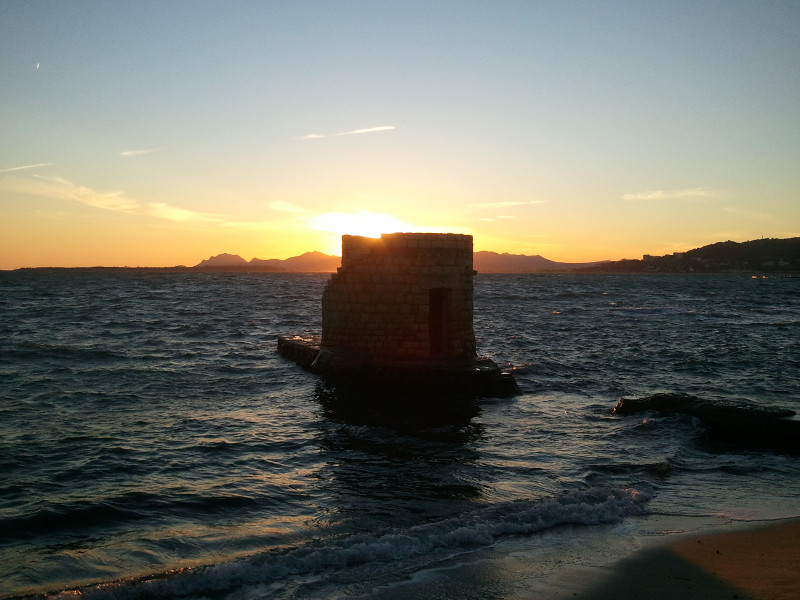
\includegraphics[width=\linewidth]{Antibes}
					\caption{Photo du Cap d'Antibes}
					\label{sub:Antibes}
				\end{subfigureth}
				\begin{subfigureth}{0.4\textwidth}
					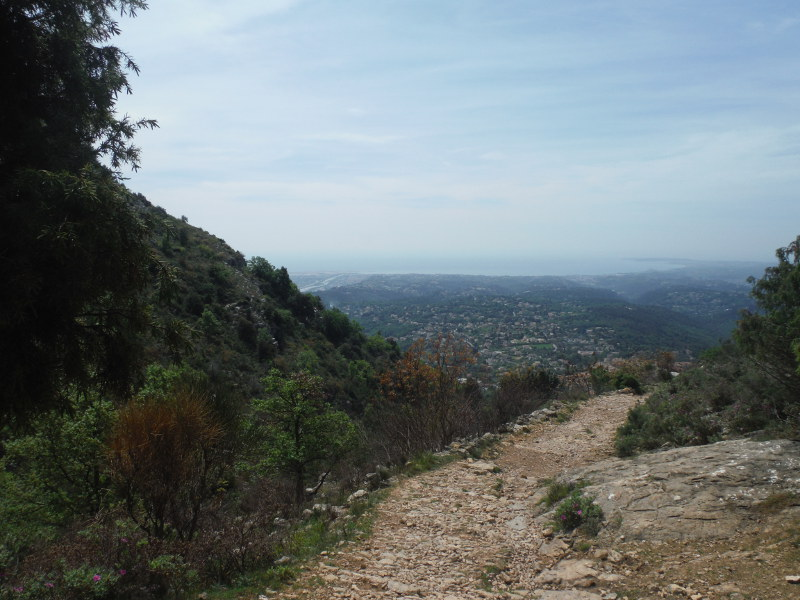
\includegraphics[width=\linewidth]{SaintJeannet}
					\caption{Saint Jeannet, depuis son Baou}
					\label{sub:SaintJeannet}
				\end{subfigureth}
				\caption[Légende courte pour la figure]{Exemple d'utilisation des sous-figures. J'utilise ici volontairement une légende longue.}		
				\label{fig:exemple}
			\end{figureth}
	
			\subsection{Exemple Symboles mathématiques}
			Rien de spécial à propos des math, hormis l'illustration des symboles listés en fin de document, tels \gls{alpha} ou \gls{gamma}, qui peuvent être utilisés indifféremment en mode \emph{in-line} ou dans des équations\footnote{Le lecteur notera que \texttt{hyperref} ajoute un lien cliquable sur chaque entrée des différents glossaires.} :
			\begin{equation}
				\gls{alpha}=\nicefrac{\gls{gamma}}{2}
				\label{eq:alphagamma}
			\end{equation}
			Les entrées des glossaires peuvent même être appelés dans des figures (PDF avec surcouche \LaTeX, ou Ti\textit{k}Z).
	

		\section{Deuxième paragraphe}
			\blindtext




	\chapter{Modélisation}
		\citationChap{
			The thing about quotes on the internet is that you can not confirm their validity
		}{Abraham Lincoln}
		\minitoc
		\newpage
		
		\section{Introduction}
		Pour pouvoir étudier un monument dans ces moindres détails de nombreux chercheurs s'orientent aujourd'hui vers la modélisation 3D. Effectivement, jusqu'à présent les scientifiques menaient leurs études à l'aide de plans ou de dessins en 2D ou bien de maquette à échelle réduite. Mais les outils numériques disponibles aujourd'hui comportent de nombreux avantages par rapport à ces anciennes techniques. Tout d'abord, il est possible d'obtenir les mêmes informations qu'avec les "anciennes techniques" en terme de côtes, formes, aspect. Mais en plus, à partir d'un modèle numérique unique, on peut sélectionner les informations que l'on souhaite étudier tout simplement en changeant les objets à afficher, les vues ou les modes d'affichage. On peut par exemple afficher un monument par vu du dessus avec ses cotes et étudier le plan 2D correspondant. Mais on peut également réaliser une impression 3D pour en avoir une maquette à l'échelle réduite. Un seul outil permet donc d'obtenir l'ensemble des informations que l'on souhaitait acquérir par le passé. Un modèle numérique 3D peut par ailleurs être utilisé par des logiciels de calcul ou de simulation afin de tester des hypothèses physiques (écoulement de fluide, acoustique, ...) ou architecturale (portance, agencement de décor, ...). Il permet également de réaliser des animations (déplacement de personnages, ouverture de haut-vents, ...) ou des visites immersives grâce aux technologies de réalité virtuelle. 

Il existe bien entendu de nombreuses limites à la numérisation 3D car cette technique est relativement récente et beaucoup de développement sont en cours. La principale contrainte est la puissance de calcul des ordinateurs et leur espace de stockage qui doivent prendre en charge de très grandes quantités de données.

Pour virtualiser des monuments, il y a deux techniques principalement utilisées. La première consiste à réaliser un nuage de point à l'aide d'appareils de mesure (laser, appareils photo, ...) à la manière d'un scanner. Prenons l'exemple de la photogrammetrie qui est aujourd'hui largement répandue dans la restitution numérique de monument. Il s'agit de photographier l'ensemble du bâtiment sous tous ses angles en s'assurant que chaque photo a une partie commune avec une autre. Les logiciels de traitement peuvent alors corréler les photos les unes avec les autres et recréer l'image en trois dimensions. Cependant, la limite de cette technique est que plus la précision est grande, plus le volume de donnée à traiter est conséquent et rend les calculs difficiles. C'est pourquoi nous avons utiliser la deuxième méthode dite de CAO (conception assistée par Ordinateur). Il s'agit de retranscrire par des formes géométriques 3D plus ou moins complexes le monuments.


		\section{Le mur de scène et ses basiliques}

Le mur de scène ainsi que ses deux basiliques constituent un bloc distinct. Le contour extérieur est créé grâce aux cotes de la planche XXI \cite{ref2}. Ce bloc est disposé dans le repère absolu d'après les cotes indiquées sur le plan nord-sud par rapport au centre de révolution de la cavea. Sur le plan est-ouest, le mur de scène extérieur (la plus grande longueur) est centré en 0, les extrémités de chacune des basiliques sont donc à 51,96m du centre.

Sont ensuite crées des objets représentant les pièces. A l'aide d'un modifier Boolean ces objets sont soustraits à la forme de base. La même méthode est utilisée pour le haut du mur qui supporte le toit (fig 24 \cite{ref},  pour les ouvertures sur le front de scène (planche XXIX \cite{ref2}), et pour les portes (planche XXI \cite{ref2}). Pour l'encastrement des poutres dans la partie sommitale du mur nous utilisons des poutres rectangulaire et identique car les traces décrites sur la planche XXXVII \cite{ref2} sont difficiles à interprétation. Cet élément pourra être corrigé par les archéologues dans une prochaine étape.

		\section{Le pulpitum et l'orchestra} 

Le pultpitum, autrement dit l'estrade de scène a complètement disparu et a aujourd'hui été remplacé par un plancher moderne. Il reste néanmoins des traces sur le mur de scène qui permettent de le modéliser dans sa version antique. Les planches XLVII et XLIX \cite{ref2} donnent les élévations du pulpitum ainsi que de l'orchestre sure les extrémités orientales et occidentales. L'orchestre est une forme volumique dont la face supérieure représente le sol. Il sera dans une prochaine étape creusé à l'aide de modifiers Boolean pour l'hyposcaenium et le caniveau décrit dans une autre partie.

		\section{La colline Saint-Europe} 
Comme souvent les architectes de l'époque ont adossé la cavea sur un relief naturel afin de solidifier la structure et de simplifier la construction de l'édifice. La colline Saint-Europe qui soutient donc le théâtre sur sa partie méridionale a été modélisée d'après les lignes d'altitude (référencées page 11 \cite{ref}) à partir de la plus basse jusqu'à la plus haute par pas de 6m par extrusion successive. Les élévation ont ensuite été légèrement adaptée (ligne par ligne) pour s'encastrer au mieux dans le théâtre. La colline est donc actuellement peu précise et il est nécessaire de l'affiner à l'aide d'un document détaillant mieux sa géométrie.

		\section{La cavea} 

La cavea est la partie semi-circulaire adossée à la colline qui soutien les maenianum (gradins). Elle comporte des ambulacres qui permettent aux spectateurs d'atteindre leur siège par le biais de vomitorium et s'ouvre sur les rues extérieures par trois étages d'arcades. La modélisation se fait à partir de la planche LX \cite{ref2} en plaçant la bordure extérieure au même niveau que la bordure des basilique (c'est à dire à 51,96m du centre). Une fois le plan de coupe réalisé on utilise un modifier Screw pour faire une extrusion circulaire autour du centre. On comprend alors que les cotes de l'ensemble de la cavea sont celles de la coupe théorique. Sur cette planche certaines valeurs sont incohérentes et on utilise donc la règle décrite en introduction de cette partie pour choisir les bonne valeurs.
Le troisième maenianum n'étant pas soutenu par la colline, il repose sur des caissons voûtés qui sont modélisés séparément. 

Les arcades donnant sur l'extérieur sont répétées à l'aide d'un modifier Array puis soustraites à la cavea par un modifier Boolean. A noter que le modifier Screw doit être appliqué pour que le Boolean fonctionne.

		\section{Maenianum} 

Les Maenianum sont modélisés à partir d'un plan de coupe d'un bloc formant un gradin auquel est appliqué un modifier Array (dupliquant du nombre de gradins) et d'un modifier Screw pour faire une extrusion de révolution. Le plan de base est un quasi-triangle représentant le profil d'un bloc rectangulaire coupé en deux. Il n'est pas coupé le long de la diagonale car une partie plate d'une dizaine de centimètre permet de faire reposer les bloc les une sur les autres. Cette forme est issue du document \cite{ref} où l'on retrouve "le seul gradin antique dont une face de joint est actuellement visible" figure \ref{coupeGradin}. C'est cette forme qui est ajustée pour coïncider avec les cotes de la cavea. Une fois les modifiers appliqués, on peut utiliser un nouveau modifier Boolean pour les marches d'escalier et les vomitorium. Les empruntes des escaliers qui seront retirés aux maenianum sont en fait la forme de base du maenianum retourné et placé de sorte que le coin supérieur (le bord du gradin) se retrouve au centre de la partie visible du gradin. Cela permet de retirer exactement la moitié de la hauteur et de la profondeur du gradin. La forme 2D de l'escalier est ensuite dupliqué avec le modifier Array et extrudé avec un modifier Solidify sur 1,2m. Cette valeur est prise arbitrairement par rapport aux plans non coté du document \cite{ref2} et devra être affinée par les experts.

		\begin{figure}[!h] %on ouvre l'environnement figure
			\center
			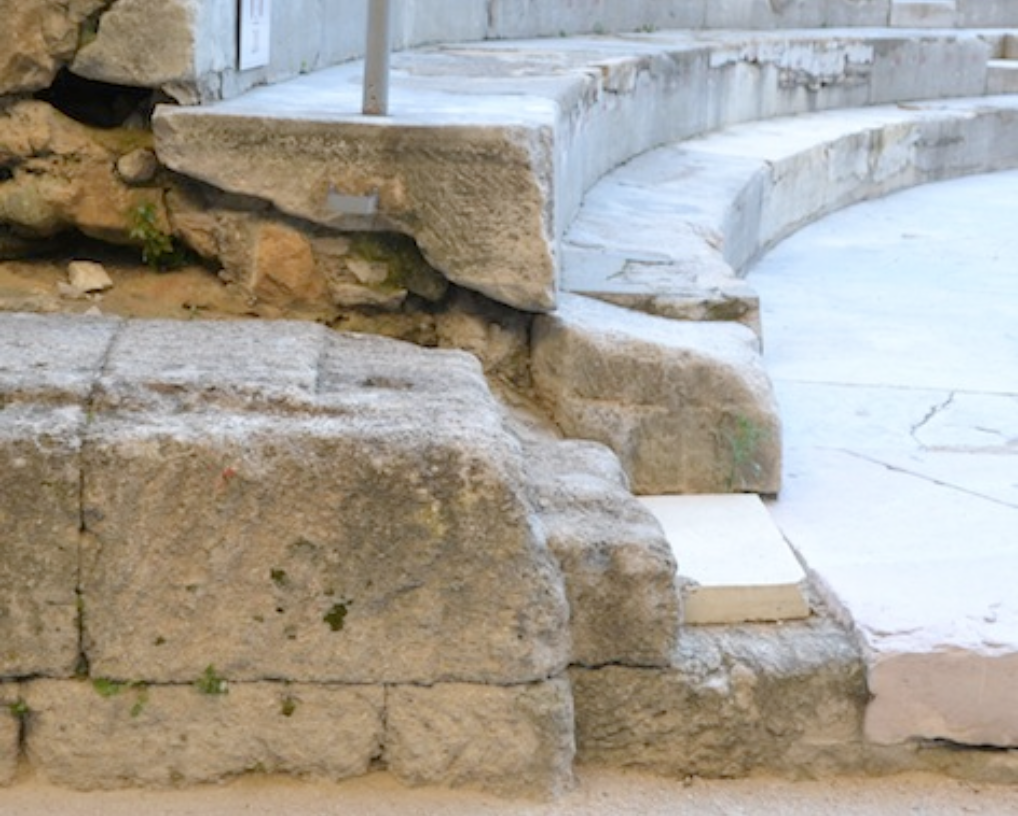
\includegraphics[scale=0.3]{images/gradinCoupe.png}
			\caption{Le repose pied et le premier gradin du premier cuneus : vu de l'extrémité nord avec au premier plan, le mur bordant l'aditus est} %la légende
			\label{coupeGradin} %l'étiquette pour faire référence à cette image	
		\end{figure} %on ferme l'environnement figure 
		
		\begin{figure}[!h] 
			\center
			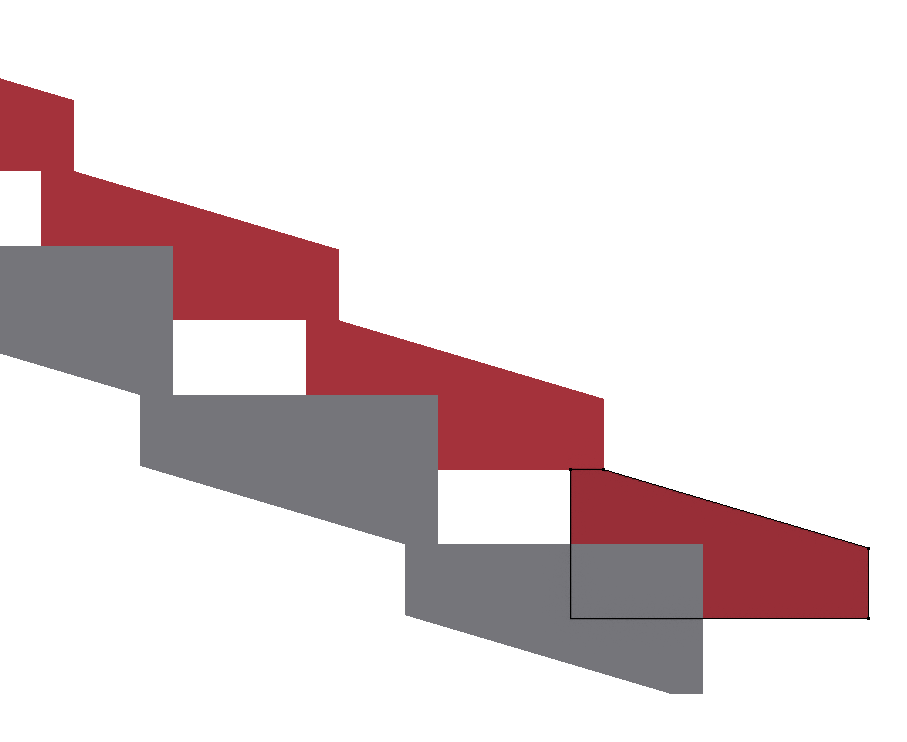
\includegraphics[scale=0.3]{images/escaliers.png}
			\caption{Modélisation des maenianum et de l'emprunte des escaliers à retirer apres application des modifers Array et Screw}
		\end{figure}
		
		\section{Aditus} 

		
	\chapter{Propositions de reconstitution}
		\citationChap{
		The thing about quotes on the internet is that you can not confirm their validity
		}{Abraham Lincoln}
		\minitoc
		\newpage
		
	\chapter*{Conclusion}
	\addcontentsline{toc}{chapter}{Conclusion}
		\newpage
			
% Biblio
%\titleformat{\chapter}[hang]{\bf\huge}{}{2pc}{} % Pour enlever "Chapitre N"
 %\titleformat{\chapter}[display]{\bf\huge}{Chapitre \thechapter}{2pc}{} % Pour remettre "Chapitre N"
 \bibliographystyle{francaissc}
 \bibliography{Part1/Biblio}
\addcontentsline{toc}{chapter}{Références}


